\clearpage
\chapter{\textit{De L'Exp\'{e}rience}}
\label{ch:experience}

\textit{De L'Exp\'{e}rience} is a composition by Tod Machover for in
in eight sections 
narrator, organ, and electronics. The piece was commissioned by the
\textit{Orchestre Symphonique de Montr\`{e}al} (OSM), and premiered at
the \textit{Maison Symphonique de Montr\'{e}al} on May 16th, 2015. The
text for the piece was taken from the writings of Michel de Montaigne,
the 16th century philosopher known for popularizing the essay form.
Performers include Jean-Willy Kunz, organist in residence with the
OSM, and narrator, Gilles Renaud. A recording of the perrmance is
available
online.\sidenote{\url{http://web.media.mit.edu/~holbrow/mas/TodMachover_OfExperience_Premier.wav}}


\subsection{The Organ}
\label{sec:organ}
The project presented a unique challenge that fits well with the
themes in this thesis. The acoustic pipe organ can project sound into
space unlike any array of loudspeakers. This is especially true for an
instrument as large and magnificent as the Pierre B\'{e}ique Organ in
the OSM concert hall, which has 6489 pipes, and extends to
approximately 10 meters above the stage. Our objective is to blend
the sound of the organ with the sound of electronics. 
% The design of the organ is a collaboration between
% Diamond Schmitt Architects and Quebec-based organ manufacturer
% Casavant.

\begin{figure*}[]
  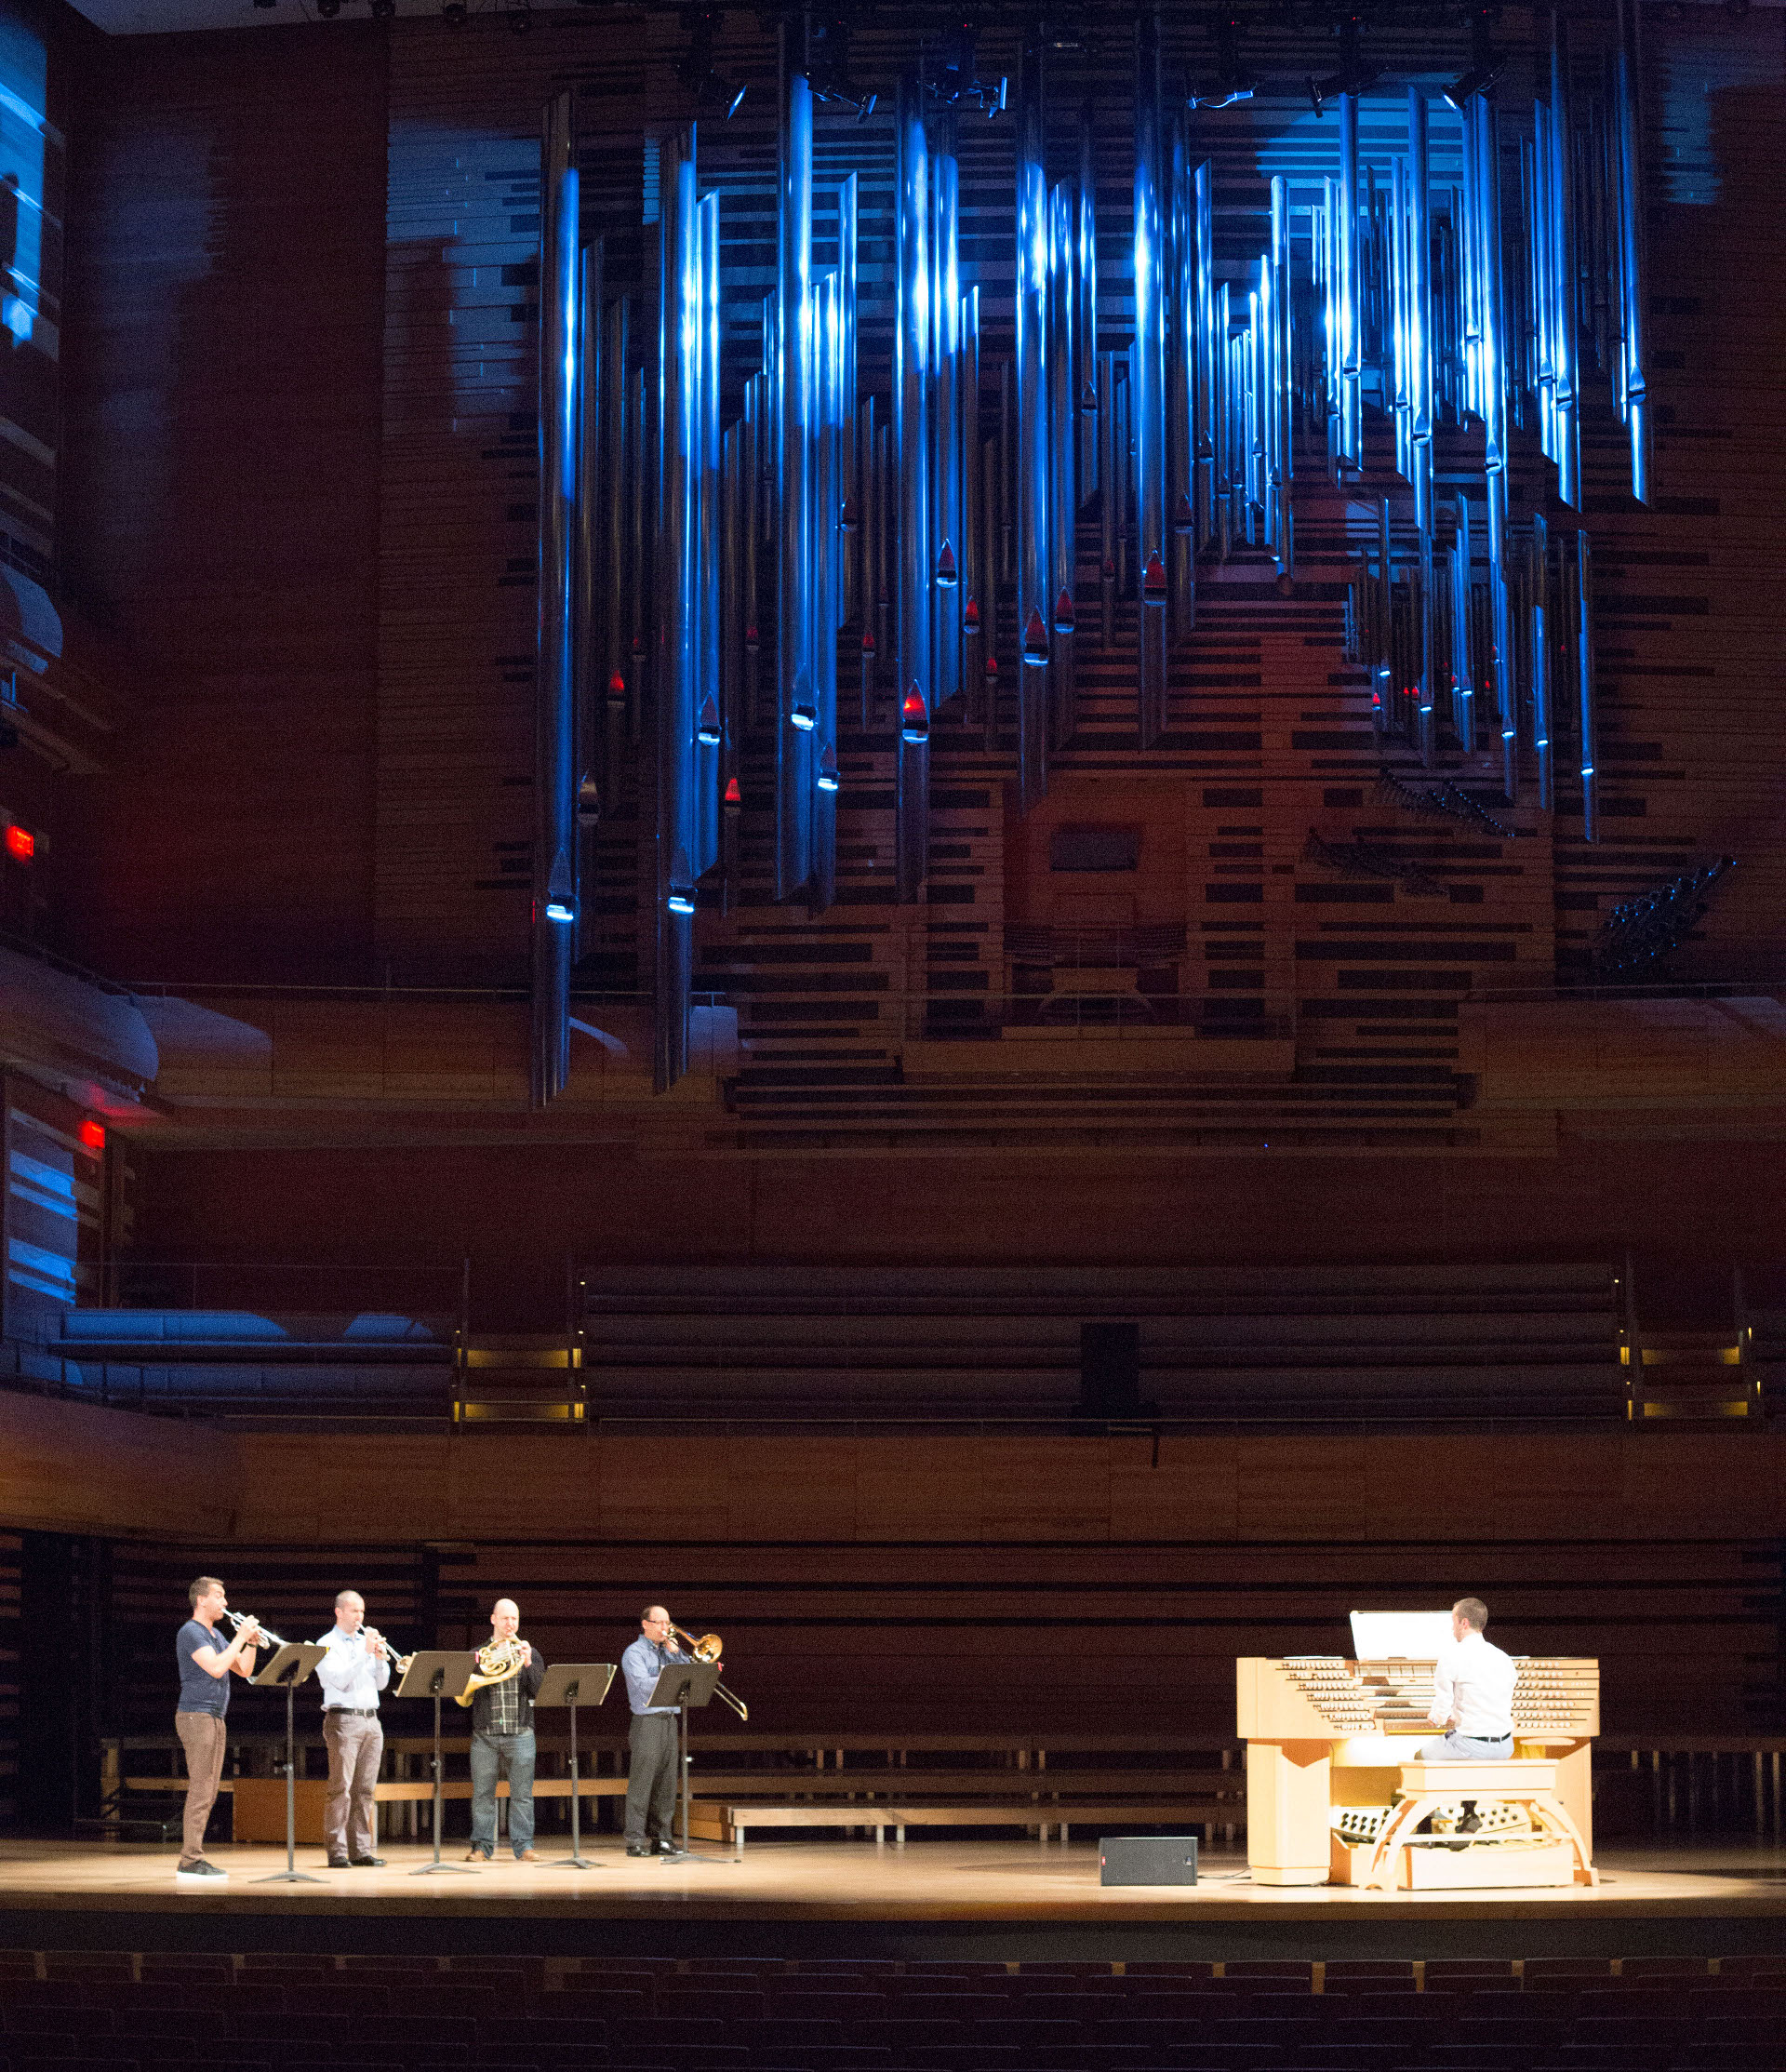
\includegraphics[width=\linewidth]{DressRehersal.jpg}
  \caption{The Pierre B\'{e}ique Organ in the OSM concert hall during
    a rehersal on May 15th, 2015. Approximately 97\% of the organs'
    6489 pipes are out of sight behind the woodwork. Photo credit: Ben
    Bloomberg}
  \label{fig:le-corbusier-sketch}
\end{figure*}


\section{Electronics}
\label{sec:electronics}
The electronics in the peice are a mix of synthesizers, pre-recorded
acoustic cello, and other processed material from acoustic and
electronic sources, all composed by Tod Machover. Prior to the
performance, these sounds were mixed ambisonically:
\begin{enumerate}
\item Other sources are positioned in space such that each has as wide
  an image as possible, but over 
\end{enumerate}The individual
sources were positioned in space such that the each has a wide image,
but overlaps with the other sources as little as possible. More
reverberant electronic sounds were placed towards the rear, while
complex and transient textures were placed more toward the front. 

During the performance the mixed ambisonic samples and patched into
the Hypercompressor. 




\subsection{Sound Reinforcement}
\label{sec:sound-reinforcement}
Loudspeakers were positioned throughout the hall. A number of factors
went into the arrangement: audience coverage, surround coverage,
rigging availability, and setup convenience. All speakers used were by
Myer Sound.\sidenote{\url{http://www.meyersound.com/}} A single CQ-2
was positioned just behind and above the narrator, to help localize
the image of his voice.  JM-1P speakers on stage left and and stage
right were also used for the voice of the narrator, and incorporated
into the ambisoic playback system. Ten pairs of UPJ-1Ps were placed in
the hall, filling in the sides and rear for ambisonic playback, Two at
the back of the hall, mirroring the CQ-2s on stage, four on each of
the first and third balconies.  The hall features variable acoustics,
and curtains can be drawn into the hall to increase acoustic
absorbtion, and decrease reverb time. These were partially engaged,
striking a balance: The reduced reverb time improved the clarity of
amplified voice, while only marginally impacting the beautiful
acoustic deacay of the organ in the hall. The show was mixed by Ben
Bloomberg. Ambisonic playback and multitrack recording of the
performance was made possible with the help and expertiese of Fabrice
Boissin and Julien Boissinot and the Centre for Interdisciplinary
Research in Music Media and Technology (CIRMMT) at McGill University.

\Paragraph{A note on composition, performance, and engineering}
No amount of engineering can compensate for poor composition,
orchestration, or performance. A skilled engineer with the right tools
only can only mitigate shortcomings in a performance. Good engineering
starts and ends with good composition, arrangement and performance. I
am have been quite fortunate that all the musicians involved with
\textit{De L'Exp\'{e}rience} at every stage are of the highest
caliber.


%%% Local Variables:
%%% mode: latex
%%% TeX-master: "CharlesHolbrow_MAS_Thesis"
%%% End:
